\chapter{Systemy informatyczne w logistyce}
\label{c3:c3}

\section{Informatyka - czym jest ?}
	Informatyka jest rozległą dziedziną nie tyle wiedzy, co zbioru zasad oraz reguł postępowania.
	Z tego powodu należy ją rozpatrywać jako:
	\begin{itemize}
		\item samodzielną dyscyplinę naukową,
		\item narzędzie wykorzystywane przez inne nauki,
		\item gałąź techniki,
		\item przemysł wytwarzający sprzęt i oprogramowanie.
	\end{itemize}	 

	Informatyka bada i jednocześnie zajmuje się definiowaniem przepływu informacji, sposobów badania
	informacji i jej przetwarzania. Można powiedzieć, że jako dyscyplina naukowa informatyka 
	jako pierwsza z nauk zaczęła badać \textbf{prawa rządzące przetwarzaniem informacji}, czyli notabene
	tak zwanej \emph{wiedzy wtórnej}. Jednocześnie informatyka stworzyła wciąż rosnący i mający 
	ogromy potencjał rynek przemysłu komputerowego, który jednocześnie definiuje, a który 
	z drugiej strony wymusza rozwój nauki, która go stworzyła \cite{it_definition}.\\
	
	W czasach społeczeństwa, przemysłu, życie osobistego zdominowanego przez potęgę informacji, informatyka
	przestała być tylko nauką, a stała się narzędziem. Narzędzie to używane jest praktycznie wszędzie
	we wszystkich swoich odmianach i mutacjach. Nie można wyobrazić sobie dzisiaj małego osiedle sklepowego bez
	małej kasy fiskalnej, do której przecież trzeba było napisać stosowne oprogramowanie sterujące i stworzyć
	elementy fizycznej struktury. Ciężko będzie znaleźć kogoś, kto nie korzysta dzisiaj z dobrodziejstw poczty
	elektronicznej, czy też ciągle rosnące rynku usług społecznościowych. Informatyka obecna jest we
	wszystkich aspektach życia, nawet jeśli nie zdajemy sobie z tego sprawy.
\section{Znaczenie informatyki w świecie logistyków}
	
	\begin{quote}
		Największym zagrożeniem dla dzisiejszej firmy jest niezdolność do dostrzegania związku
		między dzisiejszą fikcją i jutrzejszą rzeczywistością 
		\footnote{prof. Piotr Płoszajski, sprawozdanie z III Forum Praktykantów Logistyki.\\
		\url{http://spedycje.pl/logistyka/pod_znakiem_logistyka/12003/informatyzacja_logistyki.html}}.
	\end{quote}

	Współcześnie realizowana logistyka opiera się na technologiach informatycznych i w swojej rozbudowanej
	formie, w konieczności objęcia swoim zasięgiem wielu różnorodnych problemów, byłaby po prostu instrumentem
	niewygodnym. Dzięki wsparciu nauk informatycznych, logistyka od kilkunastu, jeśli nie kilkudziesięciu lat,
	istnieje jako samodzielny byt, dawno oderwany od swojego stereotypowego kojarzenie z transportem. Głównym
	powodem takiego stanu rzeczy są \textbf{zintegrowane systemy informatyczne}, wspierające efektywne zarządzanie
	przedsiębiorstwami zarówno globalnymi, jak i lokalnymi. To co łączy wszystkie systemy informatyczne jest
	z pewnością zasada, według której system powinien wspierać procesy zachodzące w organizacji od najwcześniejszego
	możliwego momentu, do chwili, kiedy gotowy produkt / usługa zostanie dostarczona do klienta. \\
	
	Procesy logistyczne, produkcyjne, dystrybucji czy też magazynowanie znacznie różnią się od tych, jakie istniały
	w czasach wielkich rewolucji przemysłowych. Liniowe łańcuchy dostaw zastąpione zostały przez złożone siatki dostawców i odbiorców,
	działających już nie w skali powiatu lub województwa, ale w skali całego kontynentu czy też świata. Dawno
	już zniknęły proste sposoby ewidencji towarów opartych na systemie kartka papieru i długopis. Ich miejsce zajęły
	kompleksowe bazy danych wraz z równie rozbudowanymi interfejsami użytkowymi. Te i inne podobne zmiany można
	uznać za podwaliny czy też synonim znaczenia informatyki dla logistyki współczesnej. \\ 
	
	Informatyka przychodząc ze swoimi możliwościami przetwarzania danych w sposób nie tyle atomowy co uwzględniający
	skomplikowane powiązaniami między informacjami dała logistykom oręż potrzebny do modelowania 
	fizycznych związków występujących między przedsiębiorcami oraz klientami, czy też utrzymania i prowadzenia
	ewidencji wydań oraz przyjęć czy też nawet zwrotów i ostatecznie wsparcia gospodarki materiałowej \cite{IDL}.
	
\section{Pojęcie systemu informatycznego}	
	Współcześnie systemy logistyczny charakteryzują się złożonością zarówno wewnętrznych oraz zewnętrznych
	procesów przepływu zasobów materiałowych, finansowych i informacyjnych. To właśnie \textbf{przepływy informacyjne} 
	są jednym z najważniejszych filarów współczesnej logistyki.
	\begin{figure}[h]
		\centering
		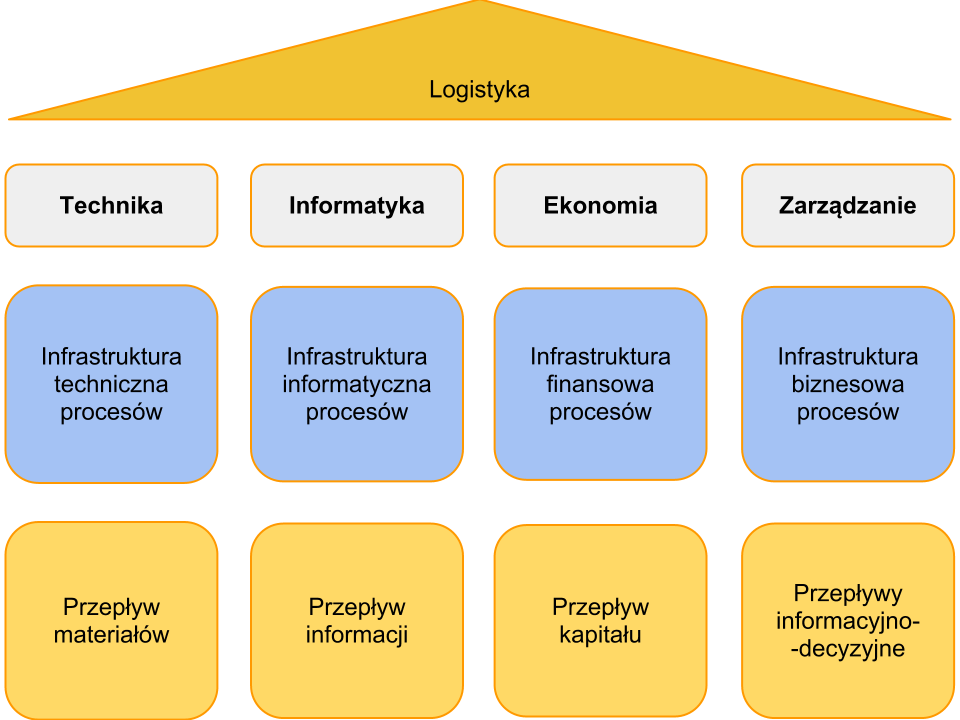
\includegraphics[width=0.95\textwidth]{images/filary_logistyki}
		\caption[Główne filary logistyki]{
			Główne filary logistyki, źródło: \cite{logistyka_w_przedsiebiorstwie}
		}
	\end{figure}
	Żyjemy dzisiaj coraz szybciej i to właśnie szybkość oraz globalizacja rynków i konkurencji
	implikujących efektywność w przetwarzania informacji wymusiły wykorzystanie odpowiednich
	systemów informatycznych, umożliwiających obieg, przetwarzanie, udostępnienia, magazynowanie
	i archiwizowanie informacji istotnych dla systemu lub jego użytkownika.  	
	
	\subsection{Czym jest system informatyczny ?}
		\begin{figure}[h]
			\label{c3:information_level_figure}
			\begin{center}
				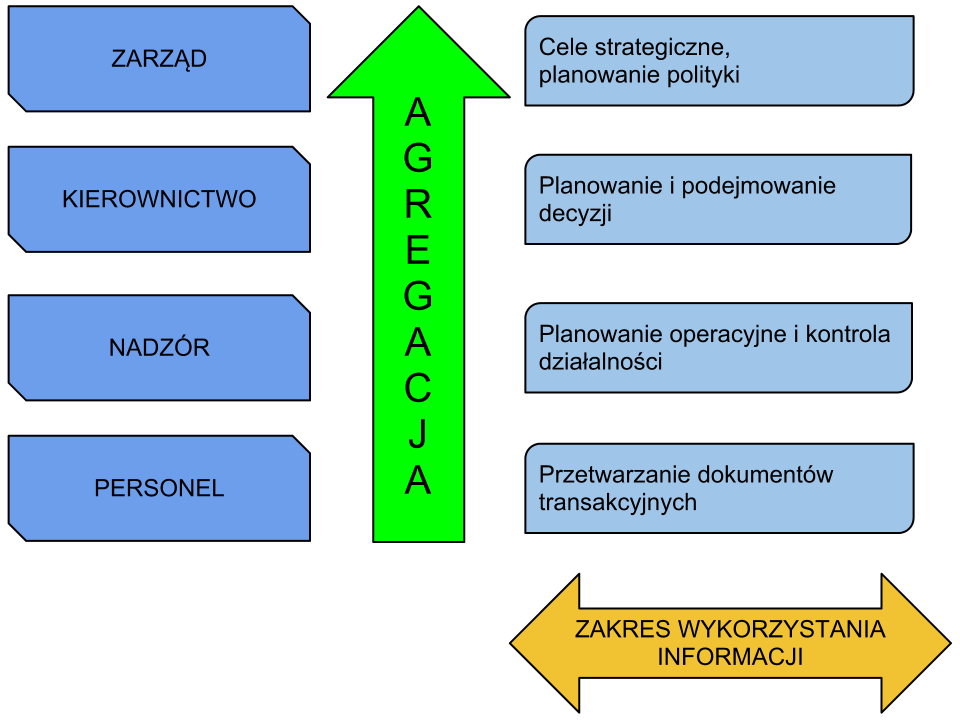
\includegraphics[width=0.95\textwidth]{images/poziomy_agregacji_informacji}
			\end{center}
			\caption[Poziomy agregacji informacji w systemie informatycznym]{
				Poziomy agregacji informacji, źródło: \cite{IDL}
			}
		\end{figure}	
	
		System informatyczny jest kompleksowym bytem, którego głównym zadaniem jest udostępnienie
		narzędzi do efektywnego przetwarzania informacji. Na system informatyczny składają się
		następujące powiązane ze sobą elementy:
		\begin{itemize}
			\item \textbf{sprzęt informatyczny} - wszelkie urządzenie informatyczne służące
			do przechowywania danych, komunikacji między modułami systemu, zestawy urządzeń
			peryferyjnych umożliwiających człowiekowi pracę z systemem lub też wszelkie urządzenie
			automatycznie kontrolowane przez system informatyczny jak np. magazyny wysokiego składu,
			\item \textbf{oprogramowanie} - zainstalowanego na komputerach z przeznaczeniem realizacji
			wyznaczonych zadań,
			\item \textbf{zasoby ludzkie} - programiści oraz osoby obsługujące komputery,
			\item \textbf{elementów organizacyjnych} - procedur korzystania z systemu informatycznego,
			\item \textbf{baz wiedzy} \cite{logistyka_w_przedsiebiorstwie}.
		\end{itemize}
		
		\paragraph{System informatyczny, czy system informacyjny ?}
		System informatyczny można traktować jako narzędzia udostępniające użytkownikom 
		obszerną funkcjonalność, pozwalającą na przetwarzanie różnych kolekcji danych.
		To właśnie dane, zapisane w bazach danych, będące niepodzielnymi faktami, są 
		spoiwem dla systemu informatycznego. Informacja jest rezultatem działania
		narzędzie wbudowanych w systemy informatyczne i wynikiem przetworzenia danych 
		atomowych z jednej postaci w inną. Uzyskujemy w ten sposób wiedzę wtórną, której można 
		użyć na różnych szczeblach zarządzania przedsiębiorstwem (rys: \ref{c3:information_level_figure}). \\
		
		Główny strumień informacji przebiega w większości przedsiębiorstw zgodnie z kierunkiem 
		\textbf{od zaopatrzenia w materiały i surowce poprzez ich magazynowanie, następnie przetworzenie ich 
		w produkty, magazynowanie produktów i sprzedaż}. Informacje te, które możemy uznać za krytyczny
		i niezbędny wspomagany jest przez informacji spływające w czasie rzeczywistym z innych działów. 
		W obszarze strumienia informacji występująca zarówno miejsca powstania kosztów, jak i zysków. 
		Systemy informatyczne stosowane do wspomagania logistyki umożliwiają bądź ułatwiają monitorowanie
		i rejestracją kosztów działania przedsiębiorstwa. 
		
	\subsection{Rodzaje systemów}
		\begin{figure}[h]
			\begin{center}
				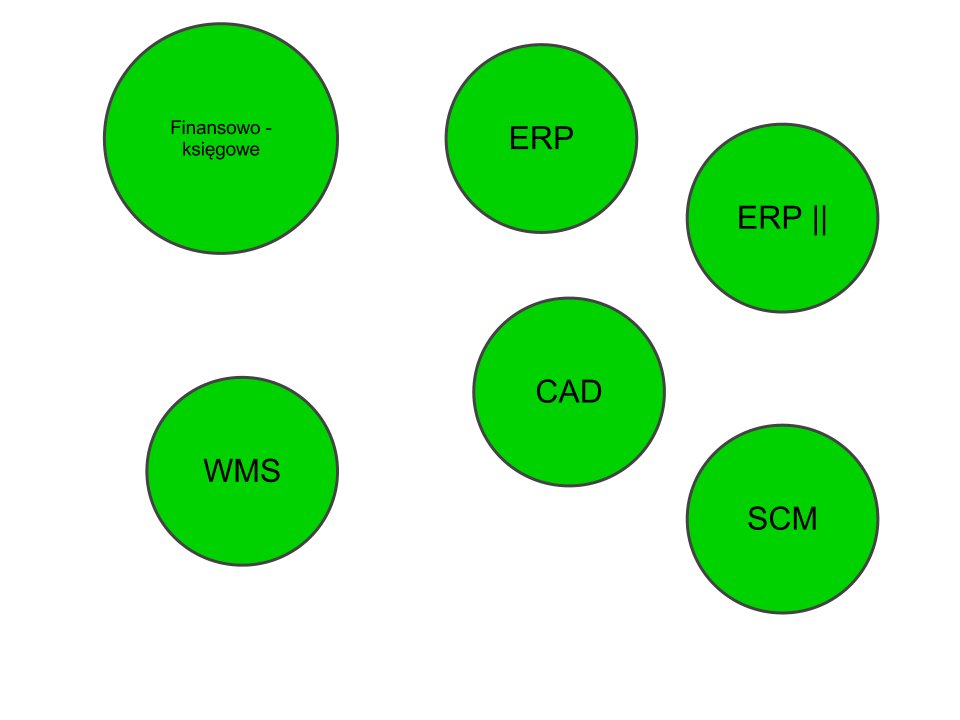
\includegraphics[width=0.95\textwidth]{images/is_logistic}
			\end{center}
			\caption[Rodzaje systemów informatycznych]{
				Rodzaje systemów informatycznych, źródło: opracowanie własne na podstawie \cite{IDL}
			}
		\end{figure}
		W kontekście omawianych systemów informatycznych do najczęściej wykorzystywanych zalicza się systemy typu
		\textbf{CAD, SCM oraz WMS}. Systemy \textbf{ERP} zalicza się do klasy wspierającej planowanie, Dzięki 
		wbudowanych algorytmach z rodziny metod typu \textbf{MRP} oraz \textbf{MRP2}. Niemniej prócz tej oczywistej
		funkcjonalności zostały one wyposażone w moduły obsługi zakupów, produkcji i sprzedaży oraz zintegrowaną
		funkcjonalnością obsługującą rozliczenia finansowo-księgowe. Wciąż nie można jednak określić takiej
		konstrukcji jako pełnoprawnego systemu SCM. Jest to spowodowane tym, że wymienione właśnie części składowe
		opierają się o przetwarzanie danych silnie związanych z produkcją, zamówieniami oraz sprzedażą. Pomijana 
		jest tutaj część przedsiębiorstwa logistycznego, bez której w ogóle nie mogłoby ono funkcjonować.
		Zastosowanie systemów z rodziny WMS oraz wbudowanych w nie algorytmów, takich jak:
		\begin{itemize}
			\item \textbf{analiza ABC} - polega na podzieleniu dóbr zaopatrzeniowych na 3 grupy według ich właściwego zużycia materiałowego.
			\item \textbf{analiza XYZ} - odwrotność metody ABC. Polega ona na podzieleniu zapasów na grupy, które charakteryzują
			zapotrzebowanie użytkownika. W ten sposób grupa \textbf{X} opisuje te towary, na które zapotrzebowanie występuje regularnie.
			Dla zobrazowanie tego, warto nadmienić, że w grupie Z będą znajdowały się te zasoby, których zarówno zapotrzebowanie, 
			jak i dokładność prognoz są niskie 
		\end{itemize}
		
	\subsection{Wykorzystanie systemów informatycznych}
		Jeśli chodzi o systemy informatyczne stworzone specjalnie z myślą o wykorzystaniu ich w 
		w charakterze aplikacji wspomagających systemy logistyczne. Z uwagi na rosnące zapotrzebowania
		konsumenckie klientów, dostawcy wciąż szukają nowych dróg doskonalenia się, ciągłego podnoszenia
		swojej konkurencyjności na rynku. Jednym z elementów tego podejścia są właśnie systemy informatyczne 
		oraz ciągle rosnąca rola informacji jako czynnika niezbędnego do właściwego działania w 
		zintegrowanych łańcuchach logistycznych. Wynikiem tego jest grupa funkcjonalności, niezależnych od
		rodzaju, czy też typu, systemu informatycznego, które zawsze są wykorzystywane przez przedsiębiorstwa,
		a bez których nie byłyby one w stanie działać w obecnej gospodarce.	
		Do tychże funkcji z pewnością należy zaliczyć:
		\begin{itemize}
			\item \textbf{gromadzenia informacji} - 
				zbieranie, rejestrowanie i ewidencjonowanie danych, które należy utożsamiać jako elementy wejściowe
				dla działającego systemy, bez których nie byłby on w stanie poprawnie realizować zleconych zadań,
			\item \textbf{przetwarzanie informacji} - 
				najczęściej sprowadza się to do realizacji podstawowych operacji
				matematycznych oraz logicznych. Niemniej warto tutaj nadmienić, że wspomniane operacje nie zawsze dotyczyć będą
				typów prostych, ale może się zdarzyć, że nastąpi konieczność przetwarzania zbiorów danych,
			\item \textbf{przechowywanie informacji} - 
				mimo, że nie jest to funkcja, którą widać na pierwszy rzut oka, jest ona z pewnością taką, bez której cały
				system nie byłby w ogóle w stanie działać. Ta oraz funkcja \emph{gromadzenia informacji} należy traktować jak wspólne
				i dopełniające się, które nie powinny działać oddzielnie. Polega na dostarczeniu odpowiedniej funkcjonalności 
				niezbędnej do zapisania informacji w sposób trwały, a także zapewnieniu, że dane nie zostaną zmienione w sposób
				niezamierzony i będą dostępne do odczytu w dowolnym momencie,
			\item \textbf{prezentowanie informacji} - 
				polega na dostarczeniu odpowiednim osobom warstwy prezentacji danych w sposób czytelny i przejrzysty, a także zgodny
				z naturą samej informacji. Ta funkcja jest częstokroć utożsamiana jako \emph{wyjście systemy informatycznego},
			\item \textbf{przesyłanie informacji} - 
				związane jest z tymi zagadnieniami, których podmiotem działania jest przesyłanie \textbf{zasobów informacyjnych}
				między jednostkami organizacyjnymi przedsiębiorstwa lub między przedsiębiorstwem a dostawcami / klientami w sposób
				zapewniający dotarcie informacji do adresata.\cite{logistyka_w_przedsiebiorstwie}.
		\end{itemize}
